
\documentclass[12pt]{article}
\usepackage[utf8]{inputenc}
\usepackage{graphicx}
\usepackage{amsmath}
\usepackage{booktabs}
\usepackage{caption}
\usepackage{subcaption}
\usepackage{geometry}
\usepackage{hyperref}
\usepackage{float}
\usepackage{enumitem}
\usepackage{xcolor}

% Page geometry
\geometry{a4paper, margin=1in}

% Hyperref settings
\hypersetup{
    colorlinks=true,
    linkcolor=blue,
    filecolor=magenta,
    urlcolor=cyan
}

% Custom commands
\newcommand{\datasetname}[1]{\textbf{#1}}
\newcommand{\paramname}[1]{\texttt{#1}}

% Title page
\begin{document}
\begin{titlepage}
    \centering
    \vspace*{2cm}

    % Logo
    
\includegraphics[width=0.4\textwidth]{scagentic_logo.png}
    \vspace{1cm}

    % Title
    \Huge\textbf{Single-Cell RNA-seq Analysis Report}
    \vspace{1cm}

    % Study information
    \Large\textbf{sample 8167, patient 1 pre-treatment biopsy, scRNA-seq}
    \vspace{0.5cm}

    % GEO accession
    \Large\textbf{GEO Accession: GSM7770556}
    \vspace{0.5cm}

    % Species and tissue
    \Large\textbf{Species: Homo sapiens}
    \vspace{0.5cm}
    \vspace{1cm}

    % Date
    \large\today
\end{titlepage}

% Table of contents
\tableofcontents
\newpage

% Study information
\section{Study Information}
\begin{itemize}
    \item \textbf{GEO Accession:} GSM7770556
    \item \textbf{Status:} Public on Sep 12, 2023
    \item \textbf{Title:} sample 8167, patient 1 pre-treatment biopsy, scRNA-seq
    \item \textbf{Source Name:} brain
    \item \textbf{Organism:} Homo sapiens
    \item \textbf{Analysis Date:} {April 04, 2025}
\end{itemize}

% Add a link to the GEO page
\begin{quote}
    \textbf{GEO Link:} \url{https://www.ncbi.nlm.nih.gov/geo/query/acc.cgi?acc=GSM7770556}
\end{quote}

% Analysis parameters
\section{Analysis Parameters}
\begin{table}[H]
    \centering
    \begin{tabular}{ll}
        \toprule
        \textbf{Parameter} & \textbf{Value} \\
        \midrule
        Min Genes & 200 \\
        Min Cells & 3 \\
        Max Percent Mt & 20 \\
        N Top Genes & 2000 \\
        N Pcs & 50 \\
        Resolution & 0.5 \\

        \bottomrule
    \end{tabular}
    \caption{Analysis parameters used in preprocessing}
    \label{tab:parameters}
\end{table}

% Analysis Pipeline
\section{{Analysis Pipeline}}

\subsection{1. Quality Control}
Calculated quality control metrics and generated distribution plots for genes, counts, and mitochondrial content. The violin plots show: (1) The number of genes expressed in the count matrix, (2) The total counts per cell, and (3) The percentage of counts in mitochondrial genes. It is useful to consider QC metrics jointly by inspecting a scatter plot colored by pct\_counts\_mt.

\begin{figure}[H]
    \centering
    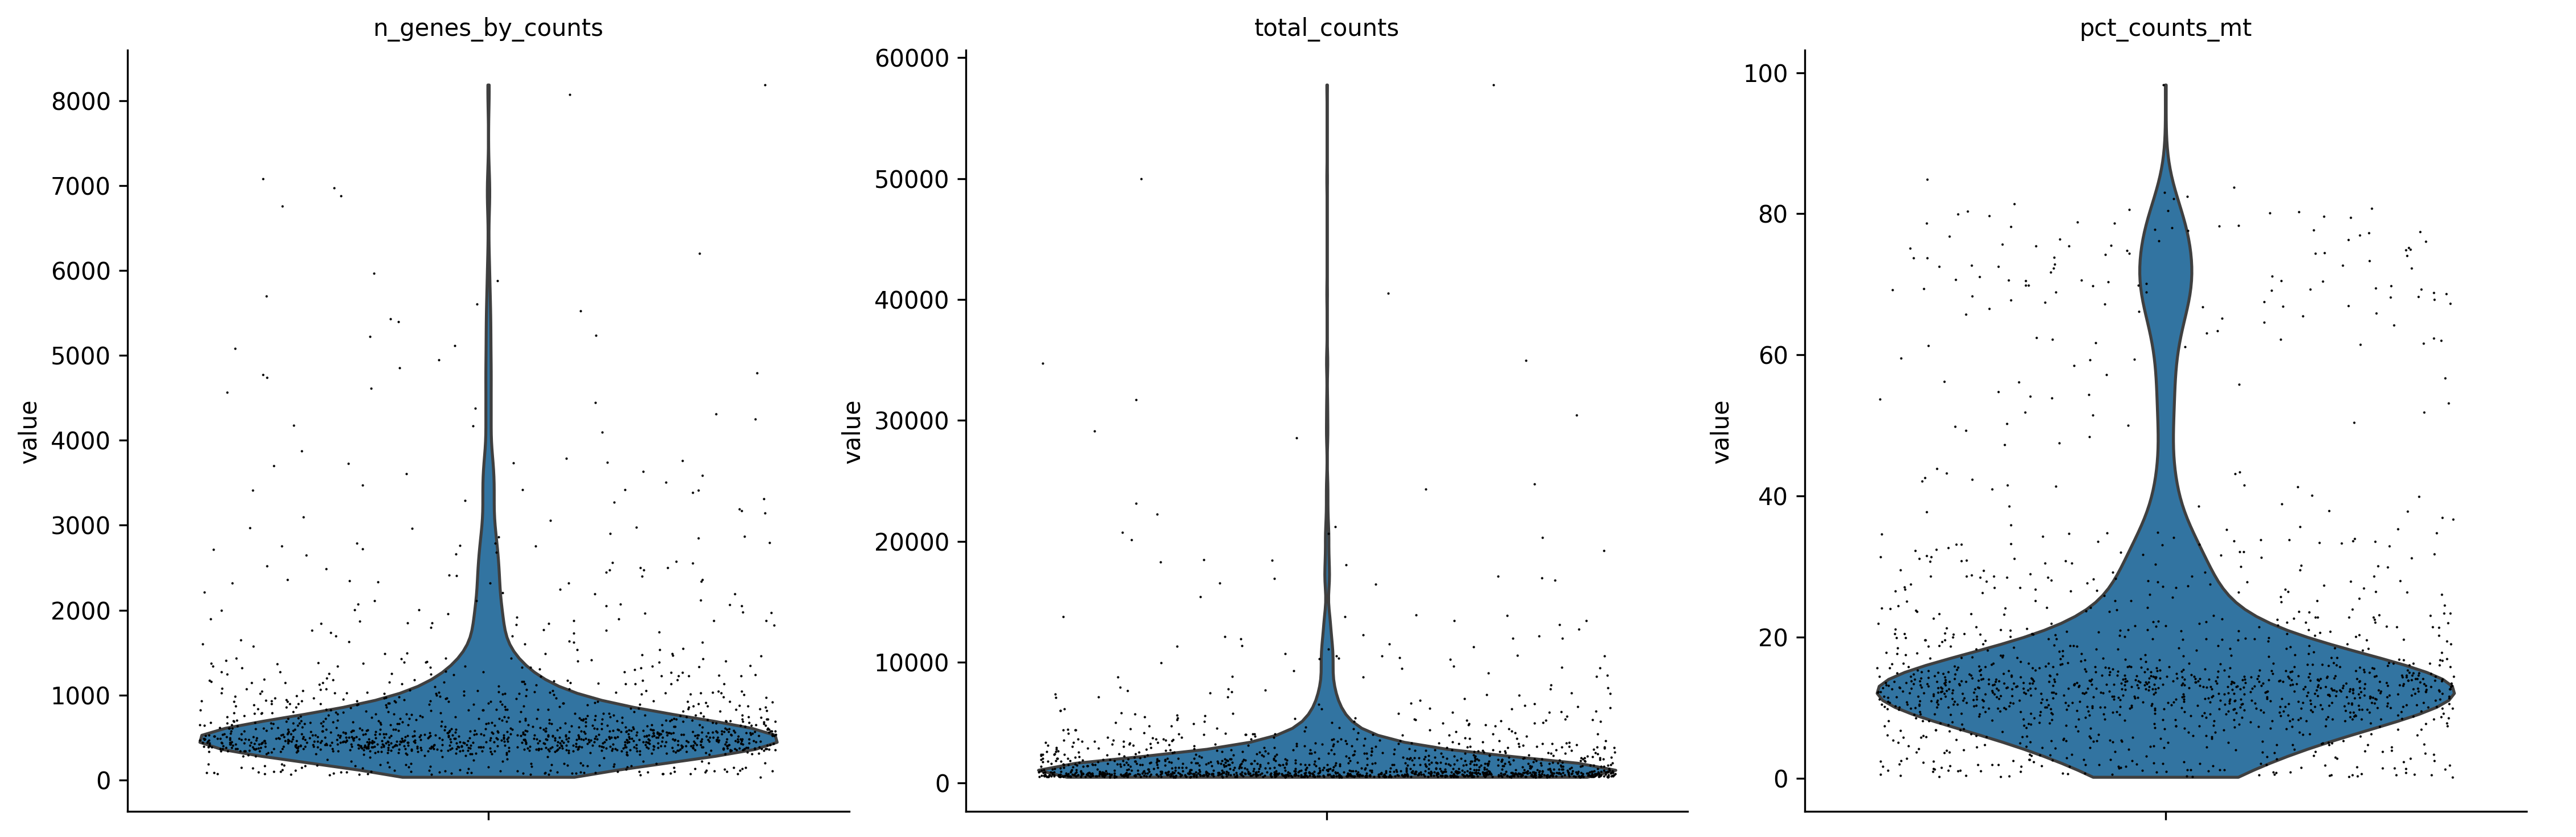
\includegraphics[width=0.8\textwidth]{qc_distributions.png}
    \caption{Quality Control}
    \label{fig:qc_distributions}
\end{figure}

\begin{figure}[H]
    \centering
    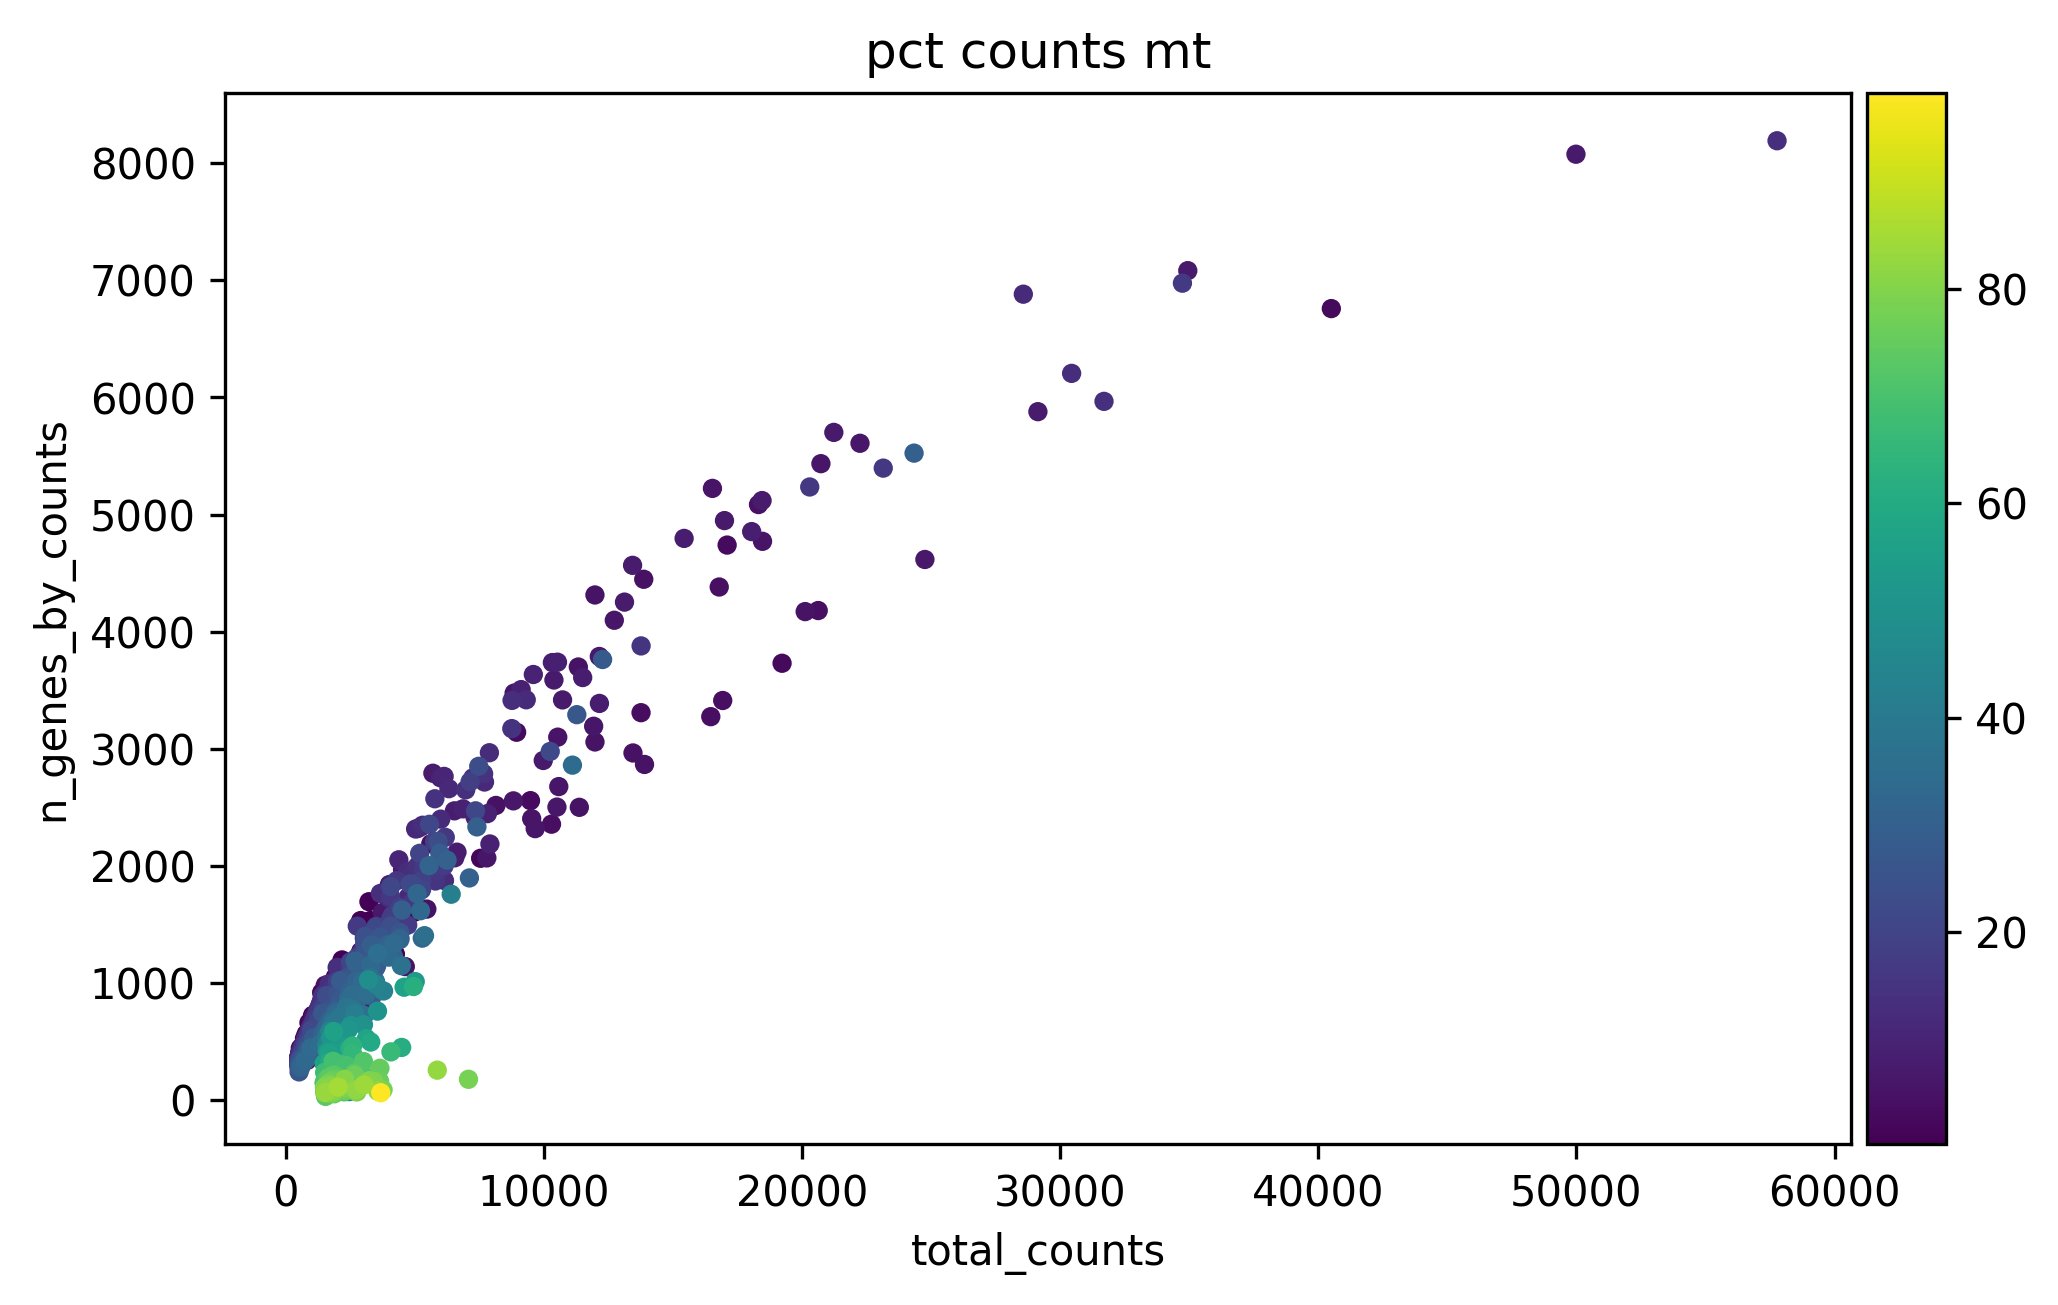
\includegraphics[width=0.8\textwidth]{qc_scatter.png}
    \caption{Additional QC visualization: Scatter plot of total counts vs. number of genes, colored by mitochondrial content percentage}
    \label{fig:qc_scatter}
\end{figure}

\subsection{2. Filtering Cells}
Filtered cells with at least 200 genes, genes expressed in at least 3 cells, and cells with less than 20\% mitochondrial content.

\subsection{3. Normalization and Scaling}
Normalized total counts per cell, applied log transformation, and scaled the data.

\subsection{4. Highly Variable Genes}
Identified the top 2000 highly variable genes for downstream analysis.

\begin{figure}[H]
    \centering
    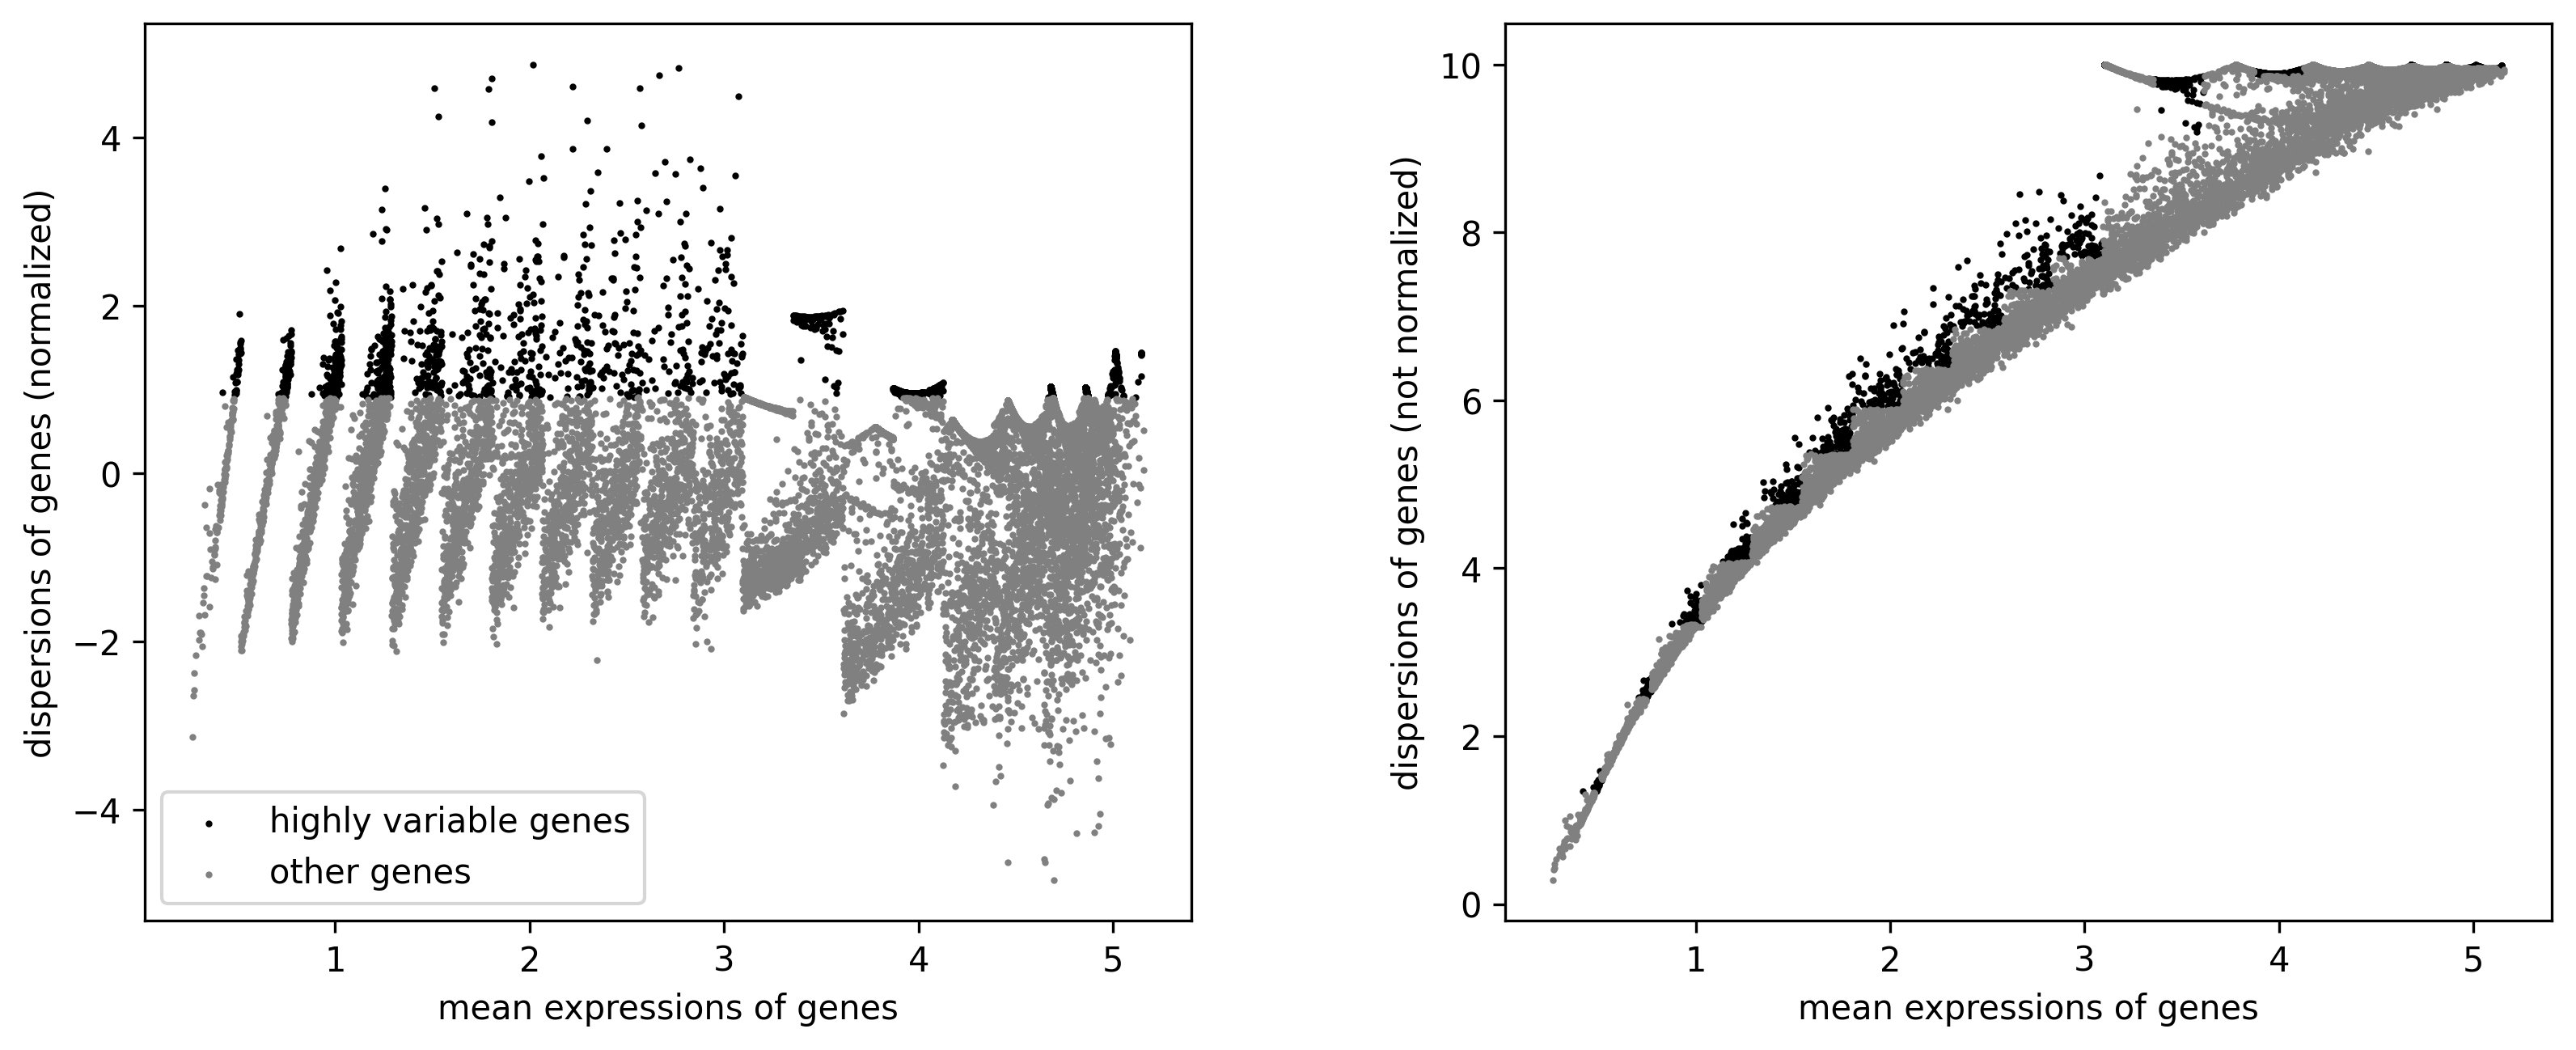
\includegraphics[width=0.8\textwidth]{highly_variable_genes.png}
    \caption{Highly Variable Genes}
    \label{fig:highly_variable_genes}
\end{figure}

\subsection{5. Principal Component Analysis}
Performed PCA on highly variable genes and visualized variance explained by the top 50 principal components.

\begin{figure}[H]
    \centering
    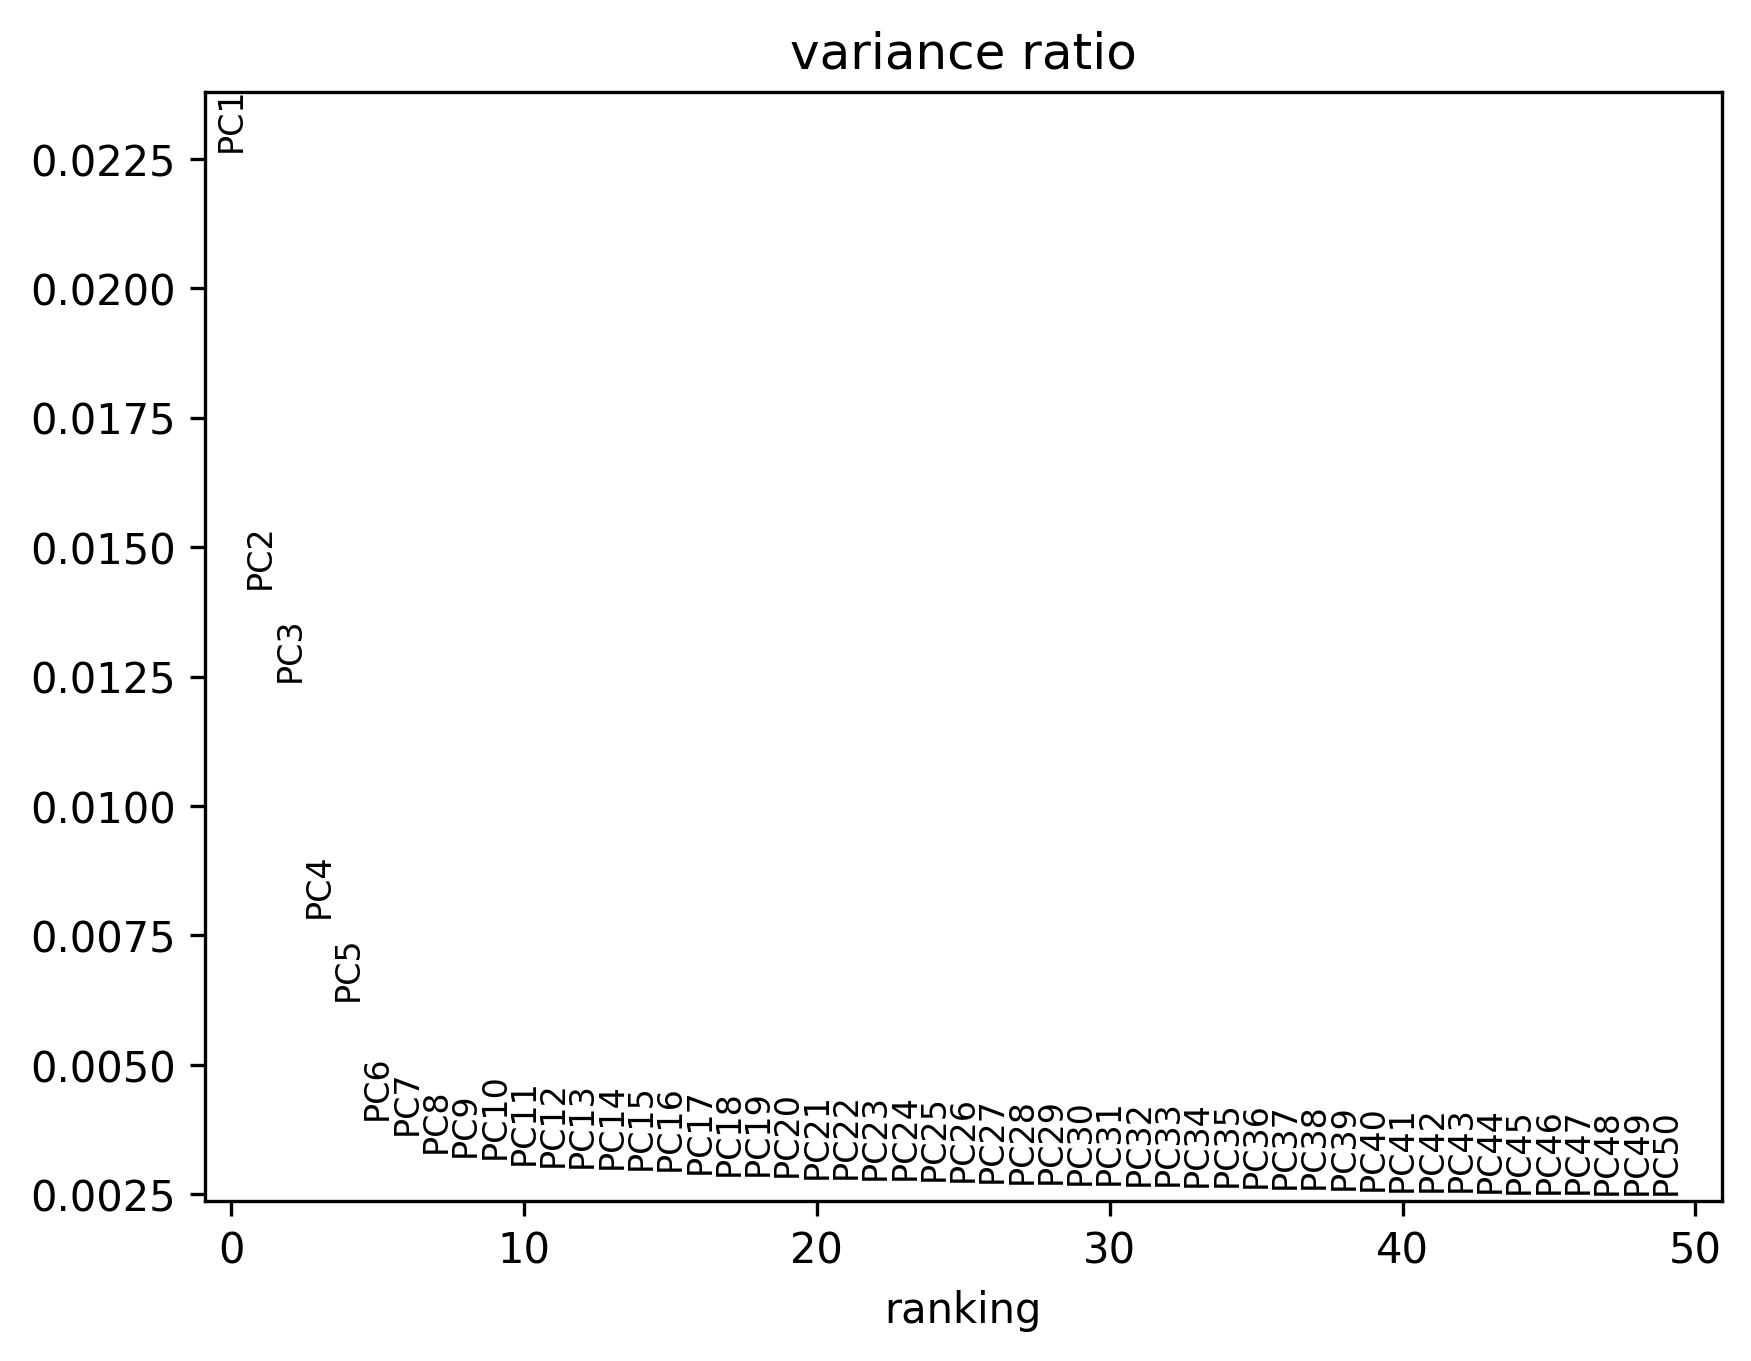
\includegraphics[width=0.8\textwidth]{pca_variance.png}
    \caption{Principal Component Analysis}
    \label{fig:pca_variance}
\end{figure}

\subsection{6. Neighborhood Graph}
Computed the neighborhood graph using 50 principal components and 10 nearest neighbors.

\subsection{7. Clustering}
Performed Leiden clustering with resolution 0.5 and visualized clusters on UMAP.

\begin{figure}[H]
    \centering
    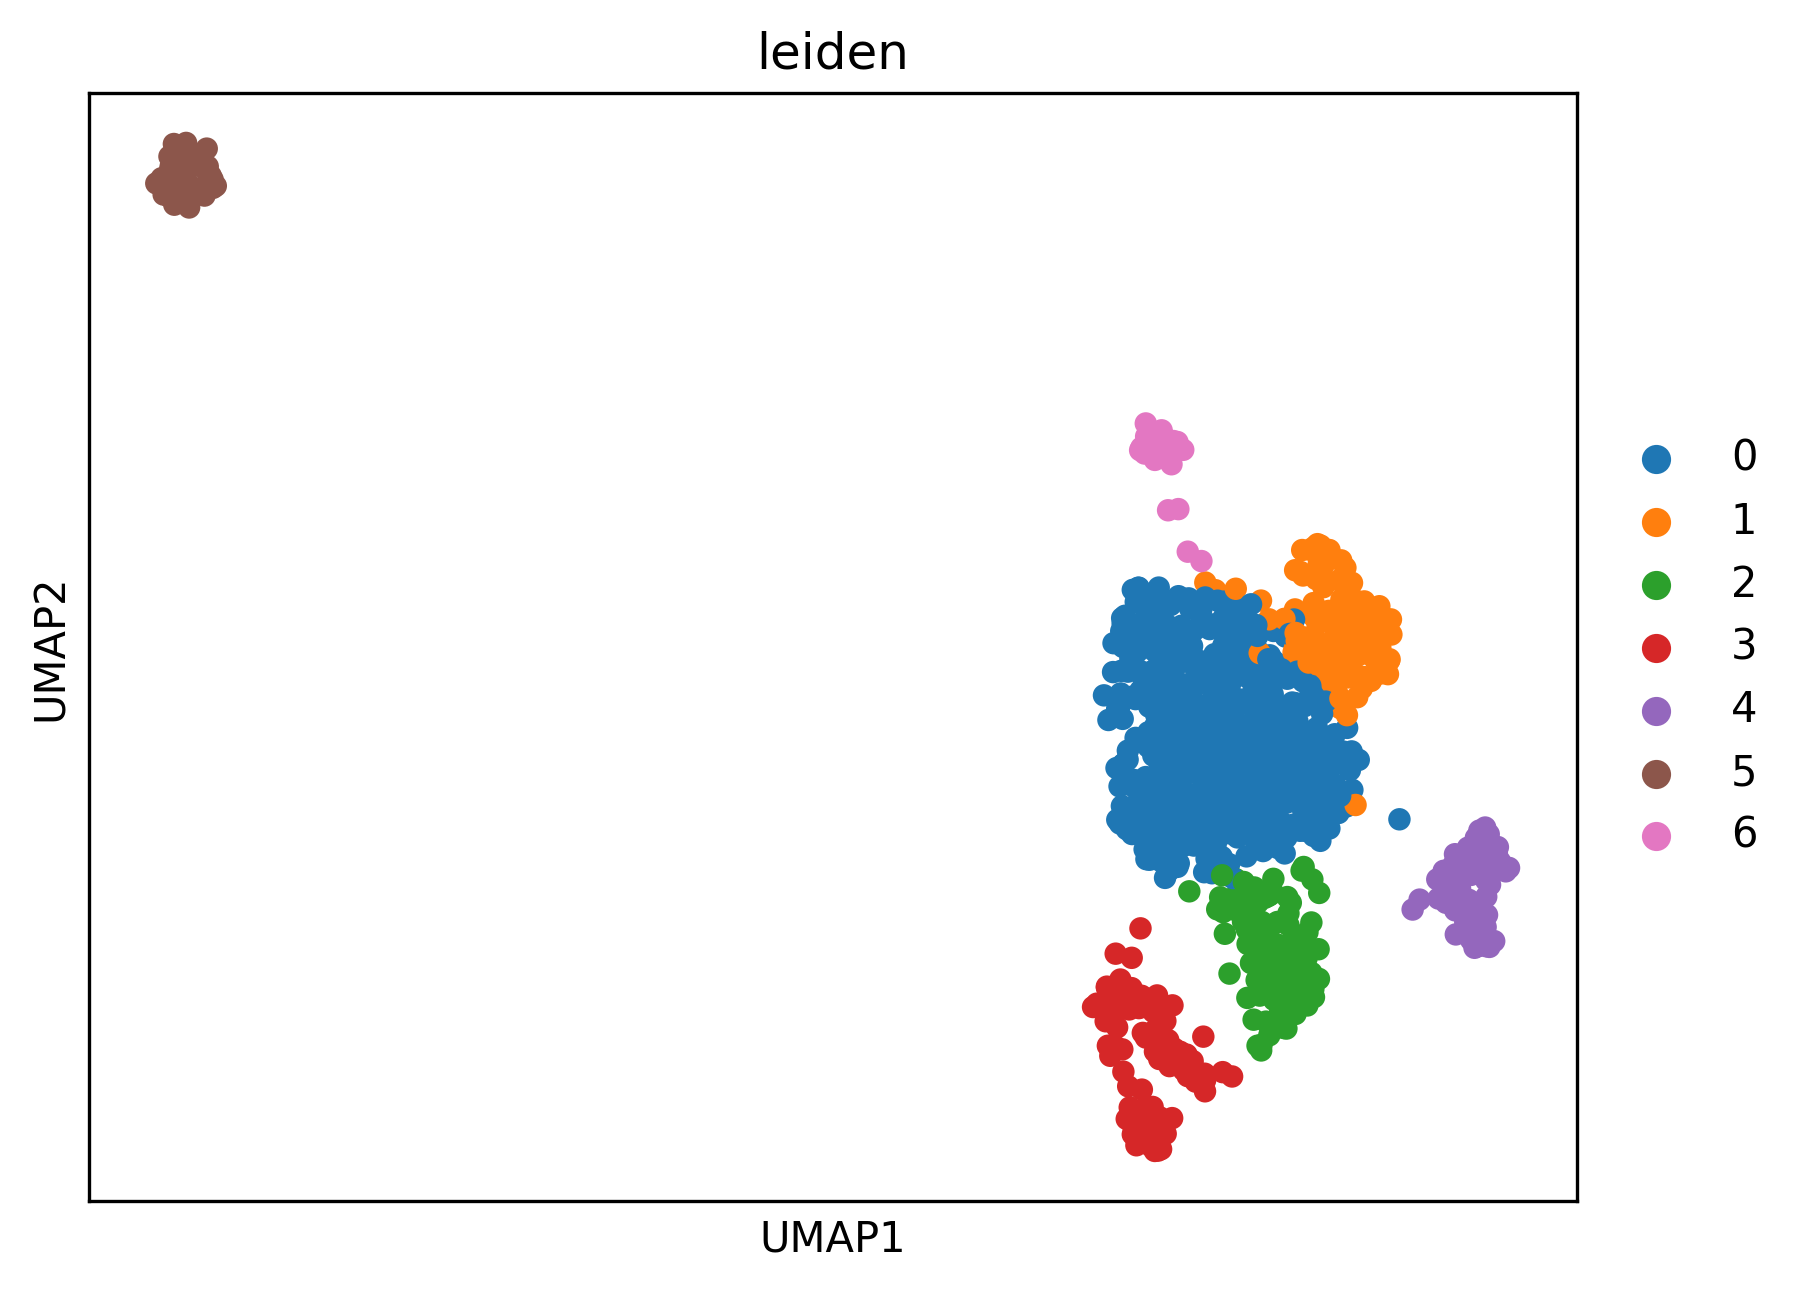
\includegraphics[width=0.8\textwidth]{umap_clusters.png}
    \caption{Clustering}
    \label{fig:umap_clusters}
\end{figure}

\subsection{8. Differential Expression Analysis}
Identified differentially expressed genes between clusters using the Wilcoxon rank-sum test.

\begin{figure}[H]
    \centering
    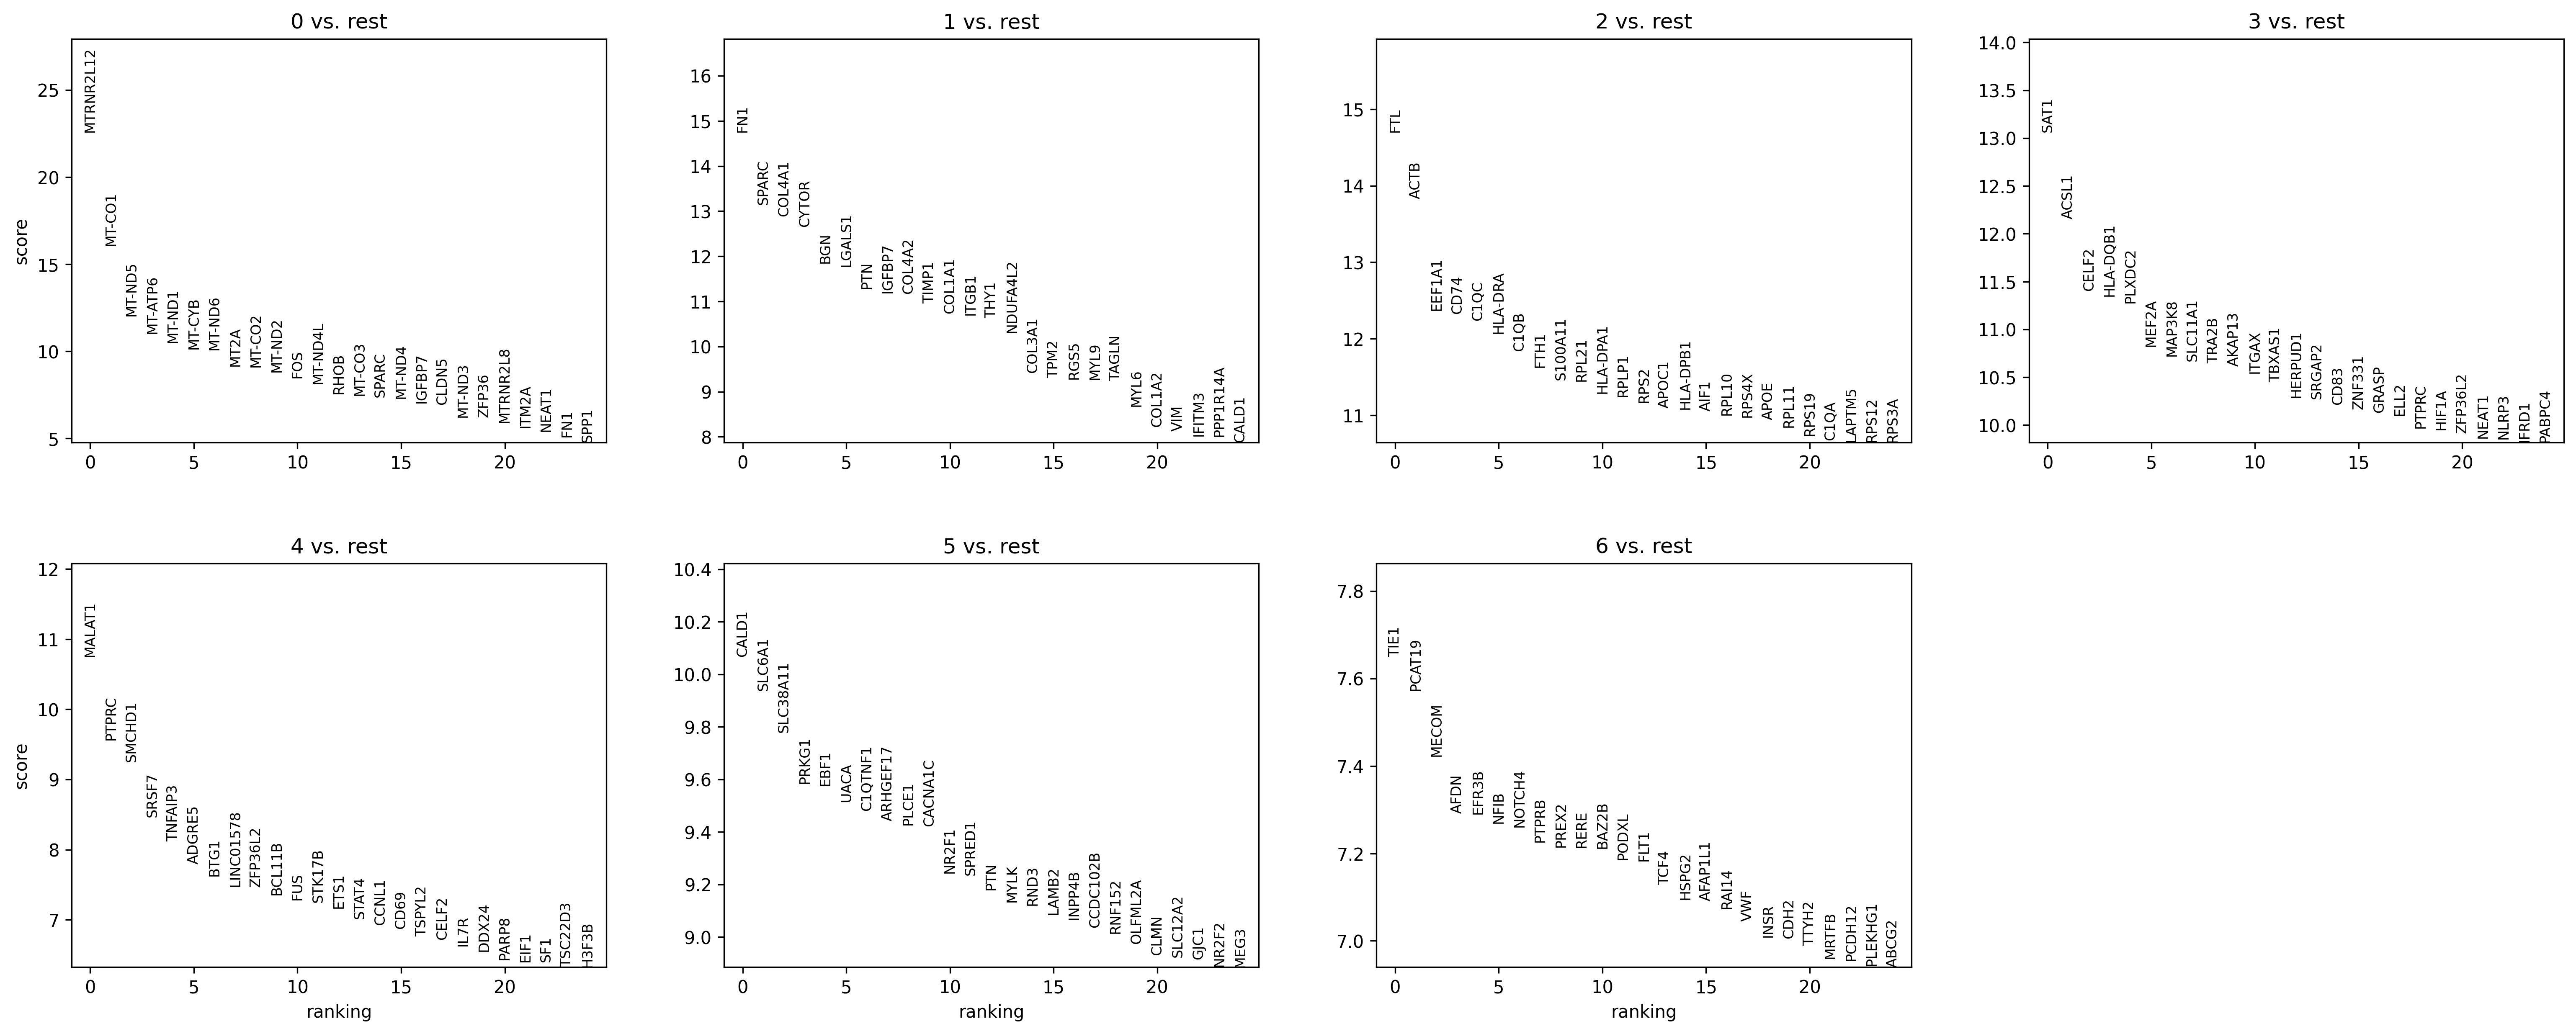
\includegraphics[width=0.8\textwidth]{de.png}
    \caption{Differential Expression Analysis}
    \label{fig:de}
\end{figure}

\end{document}
